\subsection*{(a) General DAE}
\begin{equation*}
	F(\dot x, x, \theta) = 0,\ x(0) = x_0(\theta)
\end{equation*}

Derive a differential equation for 
\begin{equation*}
	P (t) = \frac{dx(t)}{d\theta} = x_\theta
\end{equation*}

differentiating the first equation with respect to $\theta$, we get:
\begin{align*}
	\frac{dF}{d\theta} &= F_{\dot x}\,{\dot x}_\theta + F_{x}\,{x}_\theta + F_{\theta} = 0
%	\dot x_\theta &= -F_{\dot x}^{-1}\,F_{x}\,{x}_\theta - F_{\dot x}^{-1}\,F_{\theta}
\end{align*}
\subsection*{ (b) Semi-explicit DAE}
\begin{equation*}
	\dot x = F(x, y, \theta),\ x(0) = x_0(\theta), 0 = H(x,y,\theta)
\end{equation*}
differentiating the first equation with respect to $\theta$, we get:
\begin{align*}
	\dot x_p &= F_x\,x_p + F_y\,y_p + F_\theta & 0 = H_x\,x_p + H_y\,y_p + H_p
\end{align*}
\fbox{\begin{minipage}[h!]{\textwidth}
The equations for the sensitivity functions in both cases are rather similar except for the general ODE, we have the mass matrix that has to be taken into consideration. 
\end{minipage}}
\subsection*{(c) Implement sensitivity analysis for a DAE}
Reproducing the results in Section 4.3 (Figs 7-16) in the paper Timothy Maly, Linda R. Petzold, \textit{Numerical methods and software for sensitivity analysis of differential-algebraic systems}
\begin{figure}[h!b!]
	\centering
	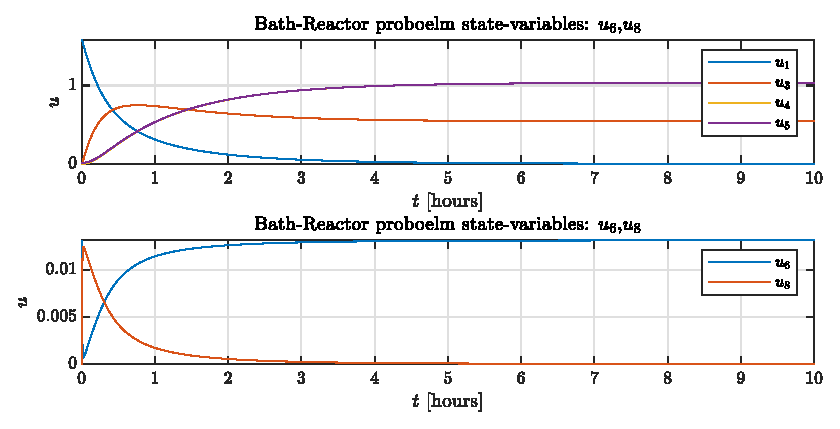
\includegraphics[width=\textwidth]{Figures/Ugf2_9c1.eps}
\end{figure}

The code for reproducing the results 
\begin{lstlisting}
%%% the initial conditions
p = [21.8893;... p1(0)
	2.14e9;... p2(0)
	32.318;... p3(0)
	21.893;... p4(0)
	1.07e9;... p5(0)
	7.65e-18;... p6(0)
	4.03e-11;... p7(0)
	5.32e-18;... p8(0)
	];
%%% the parameters
uo1 = 1.5776;
u7 = 0.5*(p(7) + sqrt(p(7)^2 + 4*p(7)*uo1)); u8 = u7;
u0 = [uo1 8.32 0 0 0 0.0131 u7 u8 0 0];


%%% the batch reactor problem
batch_reactor = @(t,u) [...
	-p(3)*u(2)*u(8)											  ;...u1'
	-p(1)*u(2)*u(6) + p(2)*u(10)     - p(3)*u(2)*u(8)         ;... u2'
	p(3)*u(2)*u(8) + p(4)*u(4)*u(6) - p(5)*u(9)               ;... u3'
	-p(4)*u(4)*u(6) + p(5)*u(9)                               ;... u4'
	p(1)*u(2)*u(6) - p(2)*u(10)                               ;... u5'
	-p(1)*u(2)*u(6) - p(4)*u(4)*u(6) + p(2)*u(10) + p(5)*u(9) ;... u6'
	-0.0131 + u(6) + u(8) + u(9) + u(10)                      ;... u7'    
	u(8)  - p(7)*u(1)/(p(7) + u(7))                           ;... u8
	u(9)  - p(8)*u(3)/(p(8) + u(7))                           ;... u9
	u(10) - p(6)*u(5)/(p(6) + u(7))                           ;... u10
];

%%% the mass matrix
M = diag([ones([1,7]) 0 0 0]);

%%% the simualtion ------------
ts = linspace(0,10,10000); % step-time of 0.001 s
options = odeset('Mass',M); % the mass matrix
[tsim,usim] = ode15s(@(t,y) batch_reactor(t,y),ts,u0,options); % BDF implicit solver
\end{lstlisting}

The Sensitivity analysis goes as follows, the code does not work but I am not sure as to why that is happening.
\begin{lstlisting}
	%% the sensitivity analysis
	% using symbolic toolbox to find out all the derivatives
	
	% clear all% temp
	
	params = sym('p',[1 8]); % parameters 
	u_syms = sym('u',[10 1]); % parameters 
	f_syms = [...
	-params(3)*u_syms(2)*u_syms(8); ...u1'
	-params(1)*u_syms(2)*u_syms(6) + params(2)*u_syms(10)     - params(3)*u_syms(2)*u_syms(8)         ;... u2'
	params(3)*u_syms(2)*u_syms(8) + params(4)*u_syms(4)*u_syms(6) - params(5)*u_syms(9)              ;... u3'
	-params(4)*u_syms(4)*u_syms(6) + params(5)*u_syms(9)                               ;... u4'
	params(1)*u_syms(2)*u_syms(6) - params(2)*u_syms(10)                              ;... u5'
	-params(1)*u_syms(2)*u_syms(6) - params(4)*u_syms(4)*u_syms(6) + params(2)*u_syms(10) + params(5)*u_syms(9) ;... u6'
	-0.0131 + u_syms(6) + u_syms(8) + u_syms(9) + u_syms(10)                      ;... u7'    
	u_syms(8)  - params(7)*u_syms(1)/(params(7) + u_syms(7))                           ;... u8
	u_syms(9)  - params(8)*u_syms(3)/(params(8) + u_syms(7))                           ;... u9
	u_syms(10) - params(6)*u_syms(5)/(params(6) + u_syms(7))                           ;... u10
	];% f_syms(t) = u_syms'(t)
	
	fp_syms = [diff(f_syms,params(1)),...
	diff(f_syms,params(2)),...
	diff(f_syms,params(3)),...
	diff(f_syms,params(4)),...
	diff(f_syms,params(5)),...
	diff(f_syms,params(6)),...
	diff(f_syms,params(7)),...
	diff(f_syms,params(8))
	]; % fp
	
	fx_syms = [diff(f_syms,u_syms(1)),...
	diff(f_syms,u_syms(2)),...
	diff(f_syms,u_syms(3)),...
	diff(f_syms,u_syms(4)),...
	diff(f_syms,u_syms(5)),...
	diff(f_syms,u_syms(6)),...
	diff(f_syms,u_syms(7)),...
	diff(f_syms,u_syms(8)),...
	diff(f_syms,u_syms(9)),...
	diff(f_syms,u_syms(10))
	]; % fx
	
	f = matlabFunction(f_syms,'Vars',[{u_syms} {params}]);
	fp = matlabFunction(fp_syms,'Vars',[{u_syms} {params}]);
	fx = matlabFunction(fx_syms,'Vars',[{u_syms} {params}]);
	
	% Xp' = Fx*Xp + Fp
	Xp0 = zeros(10,8); % initital condition
	
	Fsens = @(t,Xp) fx(interp1(tsim,usim,t,'spline')',p').*squeeze(Xp)' + fp(interp1(tsim,usim,t,'spline')',p');
	
	[tsens,Psens] = ode15s(@(t,y) Fsens(t,y),ts,Xp0);
\end{lstlisting}
